\chapter{rEDM: A Package for Empirical Dynamic Modeling Based on Attractor Reconstruction}
\label{chap_redm_package}

\definecolor{code_bg}{rgb}{0.96, 0.96, 0.96}
\lstset{language = R, upquote = true, backgroundcolor = \color{code_bg}, basewidth = 0.5em}
\lstset{basicstyle = \small\ttfamily, breaklines = true, showspaces = false, showstringspaces = false}

\section{Abstract}
Empirical dynamic modeling (EDM) is an emerging non-parametric framework for modeling nonlinear dynamic systems. In an ecological context, EDM has numerous applications, including forecasting population abundances, unraveling species interactions, and identifying causal drivers. In contrast to the conventional approach of fitting assumed model equations to data, EDM relies on the fact that ecosystems have dynamics that allows us to reconstruct attractors directly from time series. This approach (with minimal assumptions) makes EDM particularly suitable for studying ecosystems, which exhibit non-equilibrium dynamics (problematic for models that typically assume stable equilibria) and state-dependent behavior (interactions that change with system state). This guide is designed to introduce both the theory behind EDM, as well as providing practical examples for using the rEDM software package.

\section{The rEDM package}

\subsection{Installation}
rEDM is an Rcpp package, and contains both C++ and R code. Because the C++ code needs to be compiled prior to usage, there are several different options for obtaining and installing the rEDM package, depending on preference.

\subsubsection{Binary Version}
The precompiled binary version is suitable for mot users and can be downloaded from Github \href{https://github.com/ha0ye/rEDM-binary}{here}. The latest version is 0.2.6 as of August 9, 2015. Clicking on the ``view the full file'' link will initiate a downlaod of the .tgz or .zip file, which can be saved to any desired location. Note that R expects a single package file, so the downloaded archive should not be unpacked into a folder.

To install the downloaded package, the standard R command (\lstinline{install.packages}) as below, replacing \lstinline{***} with the name of the package file. (You will need to either give the complete path, or put the package file in R's current working directory.)

\begin{lstlisting}
install.packages("***", type = "source", repos = NULL)
\end{lstlisting}

Note that the Rcpp package (versions 0.11.5 and higher) must be installed first.

\subsubsection{Source Code Version}
The raw source can be downloaded from Github \href{https://github.com/ha0ye/rEDM}{here}. The package can then be built and installed following the normal procedures.

The source code is managed using Git for version control and includes an RStudio project file, so it can be cloned and built from within RStudio as well.

Finally, the package can also be installed using functions from the \emph{devtools} package:

\begin{lstlisting}
library(devtools)
install_github("ha0ye/rEDM")
\end{lstlisting}

Note that the latter two methods require the Git software to be installed. All methods here require a C++11 compiler, in addition to the Rcpp package. Installation from source has been tested using both Rtools 3.1 for Windows and XCode 5.0+ for Macintosh 10.9+.

\section{Background}

\subsection{Time Series as Observations of a Dynamic System}

The essential concept behind Empirical Dynamic Modeling (EDM) is that time series can be viewed as projections of the behavior of a dynamic system. This framework requires only a few modest assumptions:
\begin{itemize}
\item The system state can be described as a single point in a high-dimensional space. Axes can be thought of as fundamental state variables, such as population abundances, resources, or environmental properties a la the Hutchinson Niche \cite{Hutchinson_1957}.
\item The system state changes through time following some deterministic rules. In other words, the behavior is not completely random.
\end{itemize}

Projecting the system state to an axis then gives the value of the corresponding state variable, and sequential projections over time produce a time series. Different time series observed from the system can capture different state variables, but are more generally, some function of the system state and may convolve several different state variables.

\begin{figure}[!ht]
\begin{center}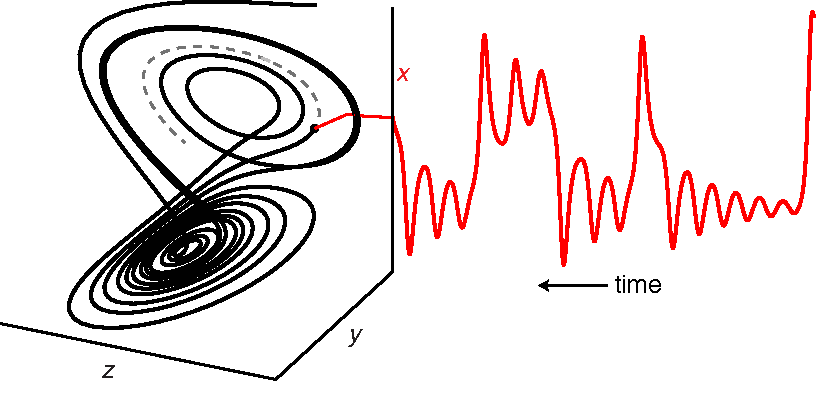
\includegraphics[width=\maxwidth{\textwidth}]{fig_redm_1.pdf}\end{center}
\caption[Time series from a dynamic system.]{\textbf{Time series from a dynamic system.}\newline
Projecting the motion of the canonical Lorenz attractor onto the $x$-axis yields a time series for variable $x$.}
\label{fig_redm_1}
\end{figure}

\subsection{Attractor Reconstruction / Takens' Theorem}

To reproduce this fundamental, geometric view of the system, one might suppose that time series of all the state variables are required. However, Takens' Theorem \cite{Takens_1981} states that a mathematically equivalent reconstruction can be created by substituting lags of a time series for the unknown or unobserved variables.

In other words, instead of representing a system state as being composed of multiple different state variables, we instead use a lagged-coordinate embedding:
$ \vec{x}_t = \langle x_t, x_{t-\tau}, \dots, x_{t-(E-1)\tau} \rangle $

\begin{figure}[!ht]
\begin{center}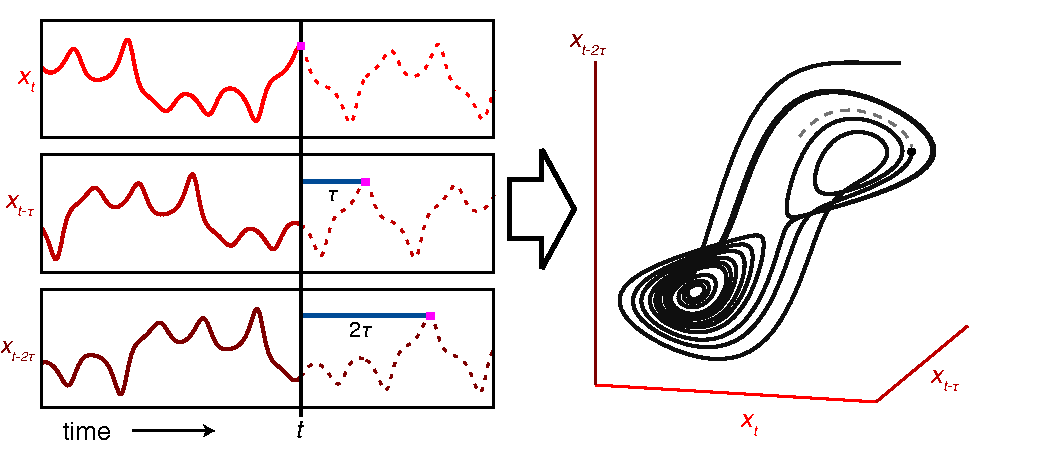
\includegraphics[width=\maxwidth{\textwidth}]{fig_redm_2.pdf}\end{center}
\caption[Attractor reconstruction from a time series.]{\textbf{Attractor reconstruction from a time series.}\newline
Successive lags (with time step $\tau$) of the time series $x_t$ are plotted as separate coordinates to form a reconstructed ``shadow'' manifold, which appears similar to the original manifold in Figure \ref{fig_redm_1}.}
\end{figure}

If sufficient lags are used, the reconstruction preserves essential mathematical properties of the original system. For instance, the points will map one-to-one to actual system states, and nearest neighbors in the reconstruction correspond to similar system states and behave similarly in the near future. 

\subsection{Nearest Neighbor Forecasting using Simplex Projection}

One application of the reconstructed attractor is prediction. This can be accomplished using nearest neighbor forecasting methods, because of the similar behavior of nearby points in the reconstruction. One such method is \emph{simplex projection} \cite{Sugihara_1990}. Simplex Projection is implemented in rEDM as the function \lstinline{simplex}, and can be used both for prediction or to identify the optimal embedding dimension by quantifying the forecast skill of reconstructions with different dimensionality.

\subsubsection{Example}

First, we load the data and look at the format. Because this dataset is part of the rEDM package, we need to first load the package into R, before we have access to its datasets and functions.

\begin{lstlisting}
library(rEDM)
data(tentmap_1d)
head(tentmap_1d)
\end{lstlisting}

\begin{lstlisting}[backgroundcolor=\color{white}, commentstyle=\ttfamily]
## [1] -0.0992003 -0.6012986  0.7998003 -0.7944096  0.7979992 -0.8195405
\end{lstlisting}

We can see that the data consists of just a single vector, containing the raw data (first-differences from a tentmap). Because the \lstinline{simplex} function can accept a single vector as the input time series, we don't need further processing of the data. Furthermore, because the data come from a discrete-time model, we can let many of the parameters be default values (e.g., $\tau = 1$, $\text{tp} = 1$). The default values for the embedding dimension, $E$, range from $1$ to $10$, and so the output will allow us to determine which embedding dimension best unfolds the attractor.

We need to specify what portions of the data to use for constructing the simplex projection model, and what portions to use for testing the forecast skill. By default, `simplex` will use leave-one-out cross-validation over the entire time series, but because the data contain no observational noise, and are particularly long, we'd like to be more conservative.

\begin{lstlisting}
lib <- c(1, 100)
pred <- c(201, 500)
\end{lstlisting}

This will use the first 100 points (time = 1 to 100) in the time series as the ``library'' to construct the model, and 300 points (time = 201 to 500) as the ``prediction set'' to test the model.

\emph{Note that if the code detects any overlap in the lib and pred, it will enable leave-one-out cross-validation and return a warning message.}

\begin{lstlisting}
ts <- tentmap_1d
simplex_output <- simplex(ts, lib, pred)
\end{lstlisting}

The results are a simple data.frame with columns for each of the model parameters and forecast statistics, and rows for each run of the model. In this case, there is one run for each value of $E$, so we can simply plot $E$ against $\rho$, the correlation between observed and predicted values:

\begin{lstlisting}
par(mar = c(4,4,1,1), mgp = c(2.5, 1, 0))
plot(simplex_output$E, simplex_output$rho, type = "l", xlab = "Embedding Dimension (E)", ylab = "Forecast Skill (rho)")
\end{lstlisting}

\begin{figure}[!ht]
\begin{center}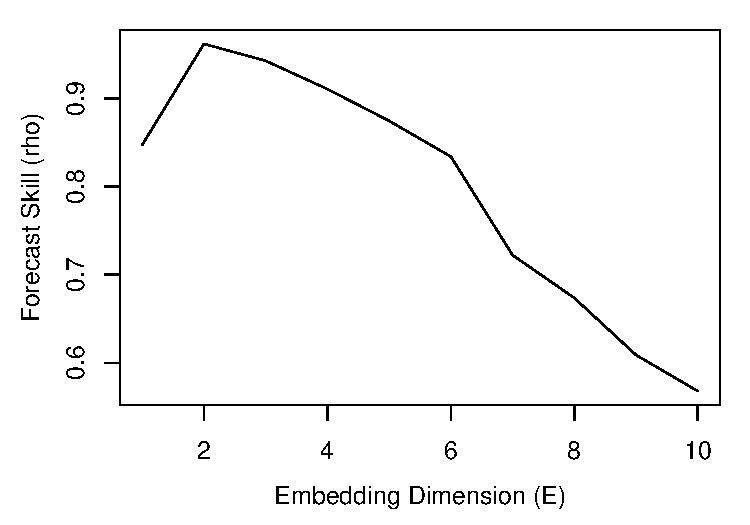
\includegraphics[width=\maxwidth{\textwidth}]{fig_redm_3.pdf}\end{center}
\caption[Identifying optimal embedding dimension using simplex projection.]{\textbf{Identifying optimal embedding dimension using simplex projection.}\newline
Plotting forecast skill ($\rho$) vs. embedding dimension ($E$) for the first-differenced tent map time series, the optimal embedding dimension is 2.}
\end{figure}

\subsection{Prediction Decay}

An important property of deterministic chaos is that nearby trajectories eventually diverge over time (the so-called ``butterfly effect''). This means that prediction is primarily limited to short-term forecasts, because over the long-term, the system state may be viewed as essentially random. This property also differentiates nonlinear systems from the equilibrium view, where the system can be expected to settle around a stable point.

\subsubsection{Example}

We can test for this property by adjusting the \lstinline{tp} parameter in the models, which determines how far into the future the model seeks to predict:

\begin{lstlisting}
simplex_output <- simplex(ts, lib, pred, E = 2, tp = 1:10)
\end{lstlisting}

Here, we can simply plot tp against $\rho$ to see how forecast accuracy changes as we predict further and further into the future:

\begin{lstlisting}
par(mar = c(4,4,1,1))
plot(simplex_output$tp, simplex_output$rho, type = "l", xlab = "Time to Prediction (tp)", ylab = "Forecast Skill (rho)")
\end{lstlisting}

\begin{figure}[!ht]
\begin{center}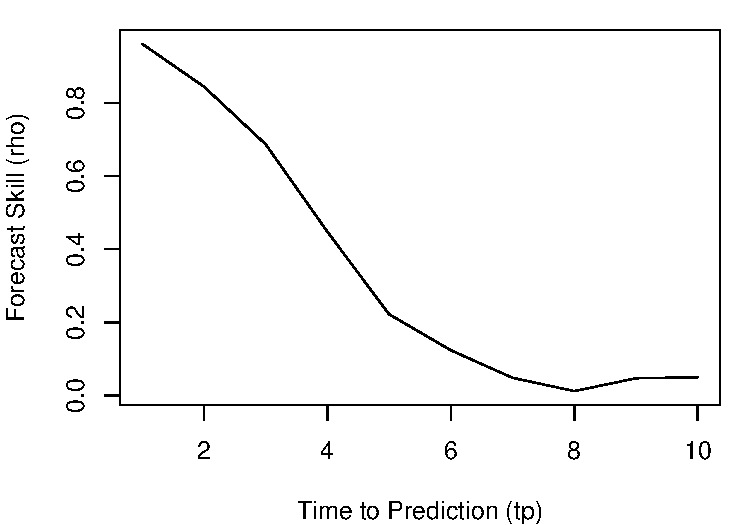
\includegraphics[width=\maxwidth{\textwidth}]{fig_redm_4.pdf}\end{center}
\caption[Identifying prediction decay using simplex projection.]{\textbf{Identifying prediction decay using simplex projection.}\newline
Plotting forecast skill ($\rho$) vs. time to prediction (tp) for the first-differenced tent map time series, predictability clearly declines with increasing forecast horizons.}
\end{figure}

\subsection{Identifying Nonlinearity}

One concern is that many time series may show predictability even if they are purely stochastic, because they behave similarly to autocorrelated red noise. Luckily, there are additional tests that can be done to distinguish between red noise and deterministic behavior, by quantifying the degree of "nonlinearity" in the data.

Here, we use the \emph{S-map} forecasting method, that is based on fitting local linear maps for prediction instead of the nearest-neighbor interpolation of simplex projection \cite{Sugihara_1994}. In addition to the parameters for simplex projection, S-map also contains a nonlinear tuning parameter, $\theta$ that affects the weights associated with individual points when fitting the local linear map. When $\theta = 0$, all weights are equal, and the S-map is identical to an autoregressive model; values of $\theta$ above $0$ give greater weight to nearby points in the state space, thereby accommodating nonlinear behavior by allowing the local linear map to vary in state-space. For autoregressive red noise, the linear model should perform better, because the S-map model can reduce observation error by averaging over many points instead of just the most nearby points.

Thus, varying $\theta$ allows us to compare equivalent linear and nonlinear models as a test for nonlinear dynamics (after first using simplex projection to estimate the optimal embedding dimension for a time-series.) 

\subsubsection{Example}

Following from the previous example, we set \lstinline{E = 2} based on the results from simplex projection. Again, note that we allow many of the parameters take on default values (e.g., $\tau = 1$, $\text{tp} = 1$). If we had changed these for simplex projection, we would want to propagate them here. The default values for the nonlinear tuning parameter, $\theta$, range from $0$ to $8$, and are suitable for our purposes.

Note also, that the default value for \lstinline{num_neighbors} is 0. Typically, when using \lstinline{s_map} to test for nonlinear behavior, we allow all points in the reconstruction to be used, subject only to the weighting based on distance. By using 0 for this parameter (an otherwise nonsensical value), the program will use all nearest neighbors.

\begin{lstlisting}
smap_output <- s_map(ts, lib, pred, E = 2)
\end{lstlisting}

Again, the results are a simple data.frame with columns for each of the model parameters and forecast statistics, and rows for each run of the model. In this case, there is one run for each value of $\theta$, so we can simply plot $\theta$ against $\rho$:

\begin{lstlisting}
par(mar = c(4,4,1,1), mgp = c(2.5, 1, 0))
plot(smap_output$theta, smap_output$rho, type = "l", xlab = "Nonlinearity (theta)", ylab = "Forecast Skill (rho)")
\end{lstlisting}

\begin{figure}[!ht]
\begin{center}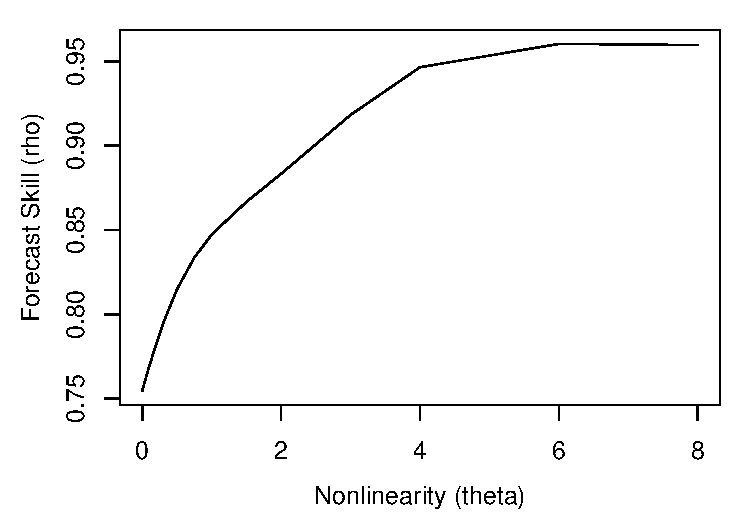
\includegraphics[width=\maxwidth{\textwidth}]{fig_redm_5.pdf}\end{center}
\caption[Identifying nonlinearity using S-map.]{\textbf{Identifying nonlinearity using S-map.}\newline
Plotting forecast skill ($\rho$) vs. nonlinearity ($\theta$) for the first-differenced tent map time series clearly shows nonlinearity, as predictability improves with $\theta > 0$.}
\end{figure}

\subsection{Generalized Takens' Theorem}

Instead of creating an attractor by taking lags of a single time series, it is possible to combine lags from different time series, if they are all observed from the same system \cite{Sauer_1991, Deyle_2011}. The practical reality of applying EDM to systems with finite data, noisy observations, and stochastic influences means that such ``multivariate'' reconstructions can often be a better depiction of the true dynamics than "univariate" counterparts.

In rEDM, the \lstinline{block_lnlp} function generalizes the \lstinline{simplex} and \lstinline{s_map} functions, allowing generic reconstructions to be used with either of the simplex projection or S-map algorithms. The main data input for \lstinline{block_lnlp} is a matrix or data.frame of the time series observations, where each column is a separate time series and each row represents the variables observed at the same time. In addition to the typical arguments for \lstinline{simplex} or \lstinline{s_map}, \lstinline{block_lnlp} contains arguments to specify which column is to be forecast (\lstinline{target_column}) as well as which columns to use to construct the attractor (\lstinline{columns}). In both cases, either a numerical index or the column name can be given. For obvious reasons, column names will work only if the input data has column names.

\emph{Note that if lagged coordinates are intended to be used, they need to be manually created as separate columns in the matrix or data.frame.}

\subsubsection{Example}

We begin by loading an example dataset of time series and lags from a coupled 3-species model system. Here, the \lstinline{block_3sp} variable is a 10-column data.frame with 1 column for time, and 3 columns for each of the variables (unlagged, t-1, and t-2 lags).

\begin{lstlisting}
data(block_3sp)
head(block_3sp)
\end{lstlisting}

\begin{lstlisting}[backgroundcolor=\color{white}, commentstyle=\ttfamily]
##  time        x_t      x_t-1      x_t-2        y_t      y_t-1      y_t-2
## 1   1 -0.7418625         NA         NA -1.2681036         NA         NA
## 2   2  1.2448818 -0.7418625         NA  1.4888875 -1.2681036         NA
## 3   3 -1.9176852  1.2448818 -0.7418625 -0.1131881  1.4888875 -1.2681036
## 4   4 -0.9623176 -1.9176852  1.2448818 -1.1067786 -0.1131881  1.4888875
## 5   5  1.3318751 -0.9623176 -1.9176852  2.3850408 -1.1067786 -0.1131881
## 6   6 -0.8170829  1.3318751 -0.9623176 -0.6753463  2.3850408 -1.1067786
##          z_t      z_t-1      z_t-2
## 1 -1.8639802         NA         NA
## 2 -0.4815825 -1.8639802         NA
## 3  1.5352388 -0.4815825 -1.8639802
## 4 -1.4929558  1.5352388 -0.4815825
## 5 -1.1194762 -1.4929558  1.5352388
## 6  0.7466579 -1.1194762 -1.4929558
\end{lstlisting}

In order to correctly index into columns, \lstinline{block_lnlp} has an option to indicate that the first column is actually a time index. When \lstinline{first_column_time} is set to \lstinline{TRUE}, a value of \lstinline{1} for \lstinline{target_column} now points to the first \emph{data} column in the data.frame, as opposed to the time column (the \lstinline{columns} parameter is similarly indexed).

\begin{lstlisting}
lib <- c(1, NROW(block_3sp))
pred <- c(1, NROW(block_3sp))

block_lnlp_output <- block_lnlp(block_3sp, lib = lib, pred = pred, columns = c(1,2,4), target_column = 1, stats_only = FALSE, first_column_time = TRUE)
\end{lstlisting}

We can also run the same model by referring to the names of the columns directly.

\begin{lstlisting}
block_lnlp_output <- block_lnlp(block_3sp, lib = lib, pred = pred, columns = c("x_t", "x_t-1", "y_t"), target_column = "x_t", stats_only = FALSE, first_column_time = TRUE)
\end{lstlisting}

Note that we did not specify a value for the \lstinline{tp} parameter. Here, the default value of \lstinline{1} means that the program will predict the target variable 1 time step into the future (based on the row-structure of the input data). In some cases, the data may already be processed into a format where one wants to predict a different column that has already been aligned correctly. In that case, one can set \lstinline{tp = 0} when calling \lstinline{block_lnlp}.

By setting \lstinline{stats_only} to \lstinline{FALSE}, we get back a list with the full model output. Only 1 model was run, so the output is a list with 1 element. To extract the raw predictions, we can go into the \lstinline{model_output} variable and pull out the observed and predicted values, plotting them to see how well the model fit relative to the expected 1:1 line.

\begin{lstlisting}
observed <- block_lnlp_output[[1]]$model_output$obs
predicted <- block_lnlp_output[[1]]$model_output$pred

par(mar = c(4,4,1,1), pty = "s")
plot_range <- range(c(observed, predicted), na.rm = TRUE)
plot(observed, predicted, xlim = plot_range, ylim = plot_range, xlab = "Observed", ylab = "Predicted")
abline(a = 0, b = 1, lty = 2, col = "blue")
\end{lstlisting}

\begin{figure}[!ht]
\begin{center}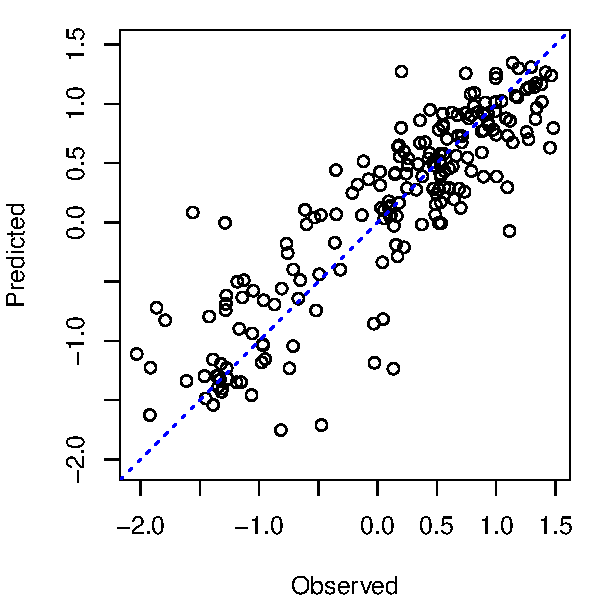
\includegraphics[width=\maxwidth{\textwidth}]{fig_redm_6.pdf}\end{center}
\caption[Forecast skill of a multivariate model.]{\textbf{Forecast skill of a multivariate model.}\newline
Predictions are plotted vs. observed values for a multivariate model for the coupled 3-species model. The dashed blue line is the one-to-one line, indicating that relatively symmetric errors.}
\end{figure}

\subsection{Causality Inference and Cross Mapping}

One of the corollaries to the Generalized Takens' Theorem is that it should be possible to cross-predict or cross-map between variables that are observed from the same system. Consider two variables, $x$ and $y$ that interact in a dynamic system. Then the univariate reconstructions based on $x$ or $y$ alone should uniquely identify the system state and the corresponding value of the other variable. Thus, it should be possible to use one variable to cross-predict the other.

\begin{figure}[!ht]
\begin{center}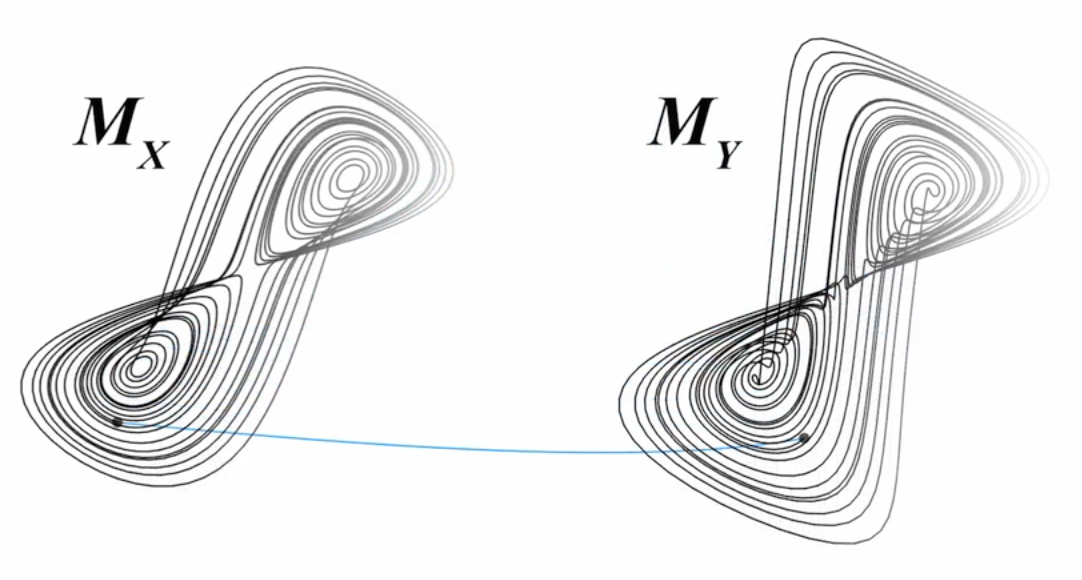
\includegraphics[width=\maxwidth{\textwidth}]{fig_redm_7.png}\end{center}
\caption[Cross mapping between two attractor reconstructions.]{\textbf{Cross mapping between two attractor reconstructions.}\newline
Reconstructions of the Lorenz Attractor using variable $x$ ($M_x$) and variable $y$ ($M_y$) map one-to-one to each other because they are both generic observations of the same dynamic system.}
\end{figure}

In the case of unidirectional causality, $x$ causes $y$, then the behavior of the causal variable ($x$) leaves a signature on the affected variable ($y$). In such cases, the reconstructed states based on $y$ can be used to cross-predict the values of $x$ (because the reconstruction based on $y$ must be complete, it must include information about the value of $x$). Note that this cross-prediction is in the \emph{opposite} direction of the causal effect. At the same time, cross-prediction from $x$ to $y$ will fail, because the time series of $x$ behaves independently of $y$, so a univariate reconstruction using only lags of $x$ is necessarily incomplete.

Although $x$ has incomplete information for predicting $y$, it does affect the values of $y$, and therefore will likely to have nonzero predictive skill. However, this cross-mapping will be limited to the statistical association between $x$ and $y$ and fail to improve as longer time series are used for reconstruction. In contrast, in the absence of noise, the cross-prediction of $x$ from $y$ will continually improve. This convergence is therefore necessary to infer causality. 

For practical reasons, the sensitivity of detecting causality this way is improved if, instead of predicting the future value of another variable, we estimate the concurrent value of another variable. We refer to this modified method as cross-mapping, because we are not ``predicting'' the future.

\subsection{Convergent Cross Mapping (CCM)}

In the rEDM package, the \lstinline{ccm} function presents an easy way to compute cross map skill for different subsamples of the time series, enabling observation of both convergence and uncertainty regarding cross map skill. In the following example, we use CCM to identify causality between anchovy landings in California and Newport Pier sea-surface temperature. 

Here, we use a previously identified value of \lstinline{3} for the embedding dimension. We set \lstinline{lib_sizes} (the number of library vectors) to vary from \lstinline{10} to \lstinline{80} in steps of \lstinline{10}. Setting \lstinline{num_samples} to \lstinline{100} means that 100 different library samples will be generated, by random sampling (\lstinline{random_libs = TRUE} by default) from the possible vectors with replacement (\lstinline{replace = TRUE} by default). 

\begin{lstlisting}
data(sardine_anchovy_sst)
anchovy_xmap_sst <- ccm(sardine_anchovy_sst, E = 3, lib_column = "anchovy", target_column = "np_sst", lib_sizes = seq(10, 80, by = 10), num_samples = 100)
sst_xmap_anchovy <- ccm(sardine_anchovy_sst, E = 3, lib_column = "np_sst", target_column = "anchovy", lib_sizes = seq(10, 80, by = 10), num_samples = 100)
\end{lstlisting}

The output from CCM is a data.frame with statistics for each model run (in this case, 100 models at each of 8 library sizes = 800 rows). Because we cross map using multiple libraries at each library size, we'd like to aggregate the results and plot the average cross map skill at each library size. Because average cross map skill less than $0$ is noninformative, we filter out negative values when plotting.

\begin{lstlisting}
a_xmap_t_means <- ccm_means(anchovy_xmap_sst)
t_xmap_a_means <- ccm_means(sst_xmap_anchovy)

par(mar = c(4,4,1,1), mgp = c(2.5, 1, 0))
plot(a_xmap_t_means$lib_size, pmax(0, a_xmap_t_means$rho), type = "l", col = "red", xlab = "Library Size", ylab = "Cross Map Skill (rho)", ylim = c(0, 0.4))
lines(t_xmap_a_means$lib_size, pmax(0, t_xmap_a_means$rho), col = "blue")
legend(x = "topleft", legend = c("anchovy xmap SST", "SST xmap anchovy"), col = c("red", "blue"), lwd = 1, inset = 0.02, cex = 0.8)
\end{lstlisting}

\begin{figure}[!ht]
\begin{center}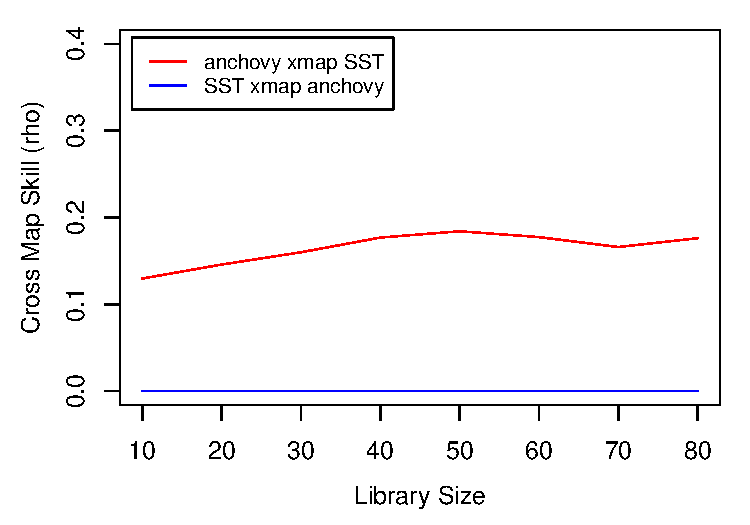
\includegraphics[width=\maxwidth{\textwidth}]{fig_redm_8.pdf}\end{center}
\caption[Causation between anchovy landings and Newport pier sea-surface temperature.]{\textbf{Causation between anchovy landings and Newport pier sea-surface temperature.}\newline
Plotting cross map skill ($\rho$) vs. library size shows clear cross mapping from anchovy to sea-surface temperature (``anchovy xmap SST''), indicating an effect of temperature on anchovy. In the converse direction (``SST xmap anchovy''), there is no cross map skill, and thus no evidence that anchovy affect temperature, as expected.}
\end{figure}

\section{Example 1: Community Productivity and Invasibility}

The data presented here are part of Experiment 120, the ``Big Biodiversity'' experiment at Cedar Creek LTER. This experiment is the longest running randomized test for the effects of plant diversity on ecosystem functions. Plots were established in 1994 and planted with 1, 2, 4, 8, or 16 species, and have since then been sampled annually for above-ground plant biomass. Full methods are described in \cite{Tilman_1997}. The most well-known result from the experiment is that planted species number strongly, positively influences above-ground biomass production. However, because the diversity treatments are fixed, rather than dynamical variables, they do not lend themselves to state space reconstruction.

Instead, we focus a different set of published results from the experiment: interactions between primary productivity, soil nitrate, and invasion rates by non-planted species. These show that increased biomass is associated with decreases in soil nitrate levels and decreases in invasion success \cite{Fargione_2005}. A posited mechanism for this is soil nitrate: increased primary productivity leads to decreased soil nitrate, which in turn reduces resources available to invaders. For the analyses here, we combine planted diversity treatments from 4-8 species planted treatments, and analyze them as a block.

The columns in the dataset \lstinline{e120_invdat} are as follows: \lstinline{Exp}, \lstinline{Year}, \lstinline{Month}, \lstinline{Plot}, \lstinline{Field}, and \lstinline{FieldPlot} describe experiment, plot identity, and sampling time. \lstinline{NumSp} and \lstinline{SpNum} show the planted and realized species diversity in the plot respectively. \lstinline{AbvBioAnnProd} shows annual aboveground productivity of planted species, in g/m$^2$. \lstinline{noh020tot} shows soil nitrate levels in the top 20 cm of soil, measured in $\mu$g/kg soil. \lstinline{invrichness} shows species richness of unplanted species in the plot. \lstinline{SummerPrecip.mm.} shows precipitation annual from May to August measured in mm.

\subsection{Preparing the Data}

E120 includes data from multiple plots, meaning that we first need to collapse it into a single composite time series. As before, we begin by normalizing each time series. 

\begin{lstlisting}
data(e120_diversity)
head(e120_diversity)

# separate time column from data
composite_ts <- e120_diversity[,c(7:9,12)]

# normalize each time series
n <- NCOL(composite_ts)
blocks <- e120_diversity$Plot
blocks_index <- sort(unique(blocks))
for(j in 1:n) {
    for(i in 1:length(blocks_index)) {
        subs <- which(blocks == blocks_index[i])
        composite_ts[subs,j] <- (composite_ts[subs,j] - mean(composite_ts[subs,j])) / sd(composite_ts[subs,j])
        }
    }

composite_ts <- cbind(year = e120_diversity$Year, composite_ts)
\end{lstlisting}

\begin{lstlisting}[backgroundcolor=\color{white}, commentstyle=\ttfamily]
##   Exp Year Month Plot NumSp SpNum AbvBioAnnProd noh020tot invrichness
## 1 120 1996     8    3     4     5       35.1670   0.22520          11
## 2 120 1997     8    3     4     5       65.9167   0.14430           7
## 3 120 1998     8    3     4     5      195.5670   0.07070           8
## 4 120 1999     8    3     4     5       69.4092   0.02610           7
## 6 120 2001     8    3     4     5       80.6292   0.18045           3
## 7 120 2002     8    3     4     5      143.5750   0.01130           9
##   Field FieldPlot SummerPrecip.mm.
## 1     1       1 3          447.548
## 2     1       1 3          445.516
## 3     1       1 3          356.108
## 4     1       1 3          487.680
## 6     1       1 3          356.870
## 7     1       1 3          484.886
\end{lstlisting}

Again, we need to indicate separations between plots so that lagged vectors are not constructed that contain coordinates spanning multiple time series.

\begin{lstlisting}
# make composite library
segments <- NULL
startpos <- 1
for(i in 2:nrow(composite_ts)) {
    if(composite_ts$year[i] < composite_ts$year[i-1]) {
        segments <- rbind(segments, c(startpos, i))
        startpos <- i+1
        }
    }
segments <- rbind(segments, c(max(segments)+1, nrow(composite_ts)))

# choose random segments for prediction
set.seed(2312)
rndlib <- sort(sample(1:nrow(segments), round(nrow(segments)/2,0), rep=FALSE))
composite_lib <- segments[rndlib,]
composite_pred <- segments[-rndlib,]
\end{lstlisting}

Because the time series for precipitation does not vary among replicates, we also need to construct separate variables for analyzing precipitation dynamics:
 
\begin{lstlisting}
precip_ts <- unique(e120_diversity[,c("Year", "SummerPrecip.mm.")])
precip_ts <- precip_ts[order(precip_ts$Year),]
\end{lstlisting}

\subsection{Applying Simplex and S-map Algorithms}

We can then use the rEDM functions as normal for each of our time series. First, we apply simplex projection:
 
\begin{lstlisting}
par(mar = c(4,4,1,1), mfrow=c(2,2), mgp = c(2.5, 1, 0))
varlst <- colnames(composite_ts)[2:4]
simplex_output_list <- NULL

for(i in 1:length(varlst)) {
    simplex_output_list[[i]] <- simplex(composite_ts[,c("year", varlst[i])], lib=composite_lib, pred=composite_pred, E = c(2:6))
    plot(simplex_output_list[[i]]$E, simplex_output_list[[i]]$rho, type = "l", xlab = "Embedding Dimension (E)", ylab = "Forecast Skill (rho)", main=varlst[i])
    }

simplex_output_list[[4]] <- simplex(precip_ts, lib = c(1,7), pred = c(1,7), E = c(2:6), silent = TRUE)
names(simplex_output_list) <- c(varlst, "precipmm")
plot(simplex_output_list[[4]]$E, simplex_output_list[[4]]$rho, type = "l", xlab = "Embedding Dimension (E)", ylab = "Forecast Skill (rho)", main="Precip")
\end{lstlisting}

\begin{figure}[!ht]
\begin{center}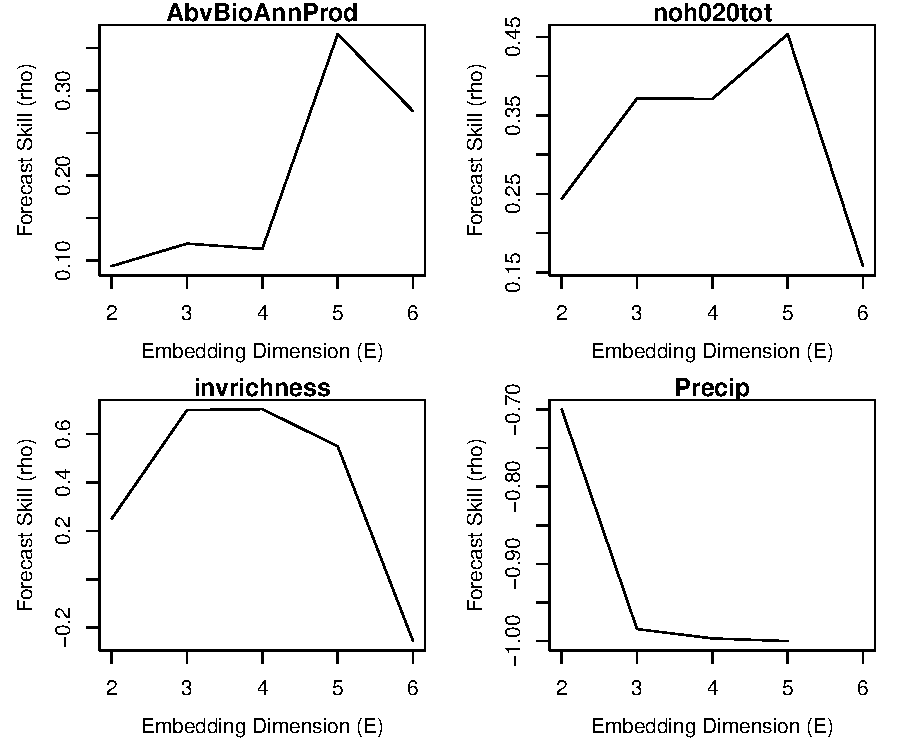
\includegraphics[width=\maxwidth{\textwidth}]{fig_redm_9.pdf}\end{center}
\caption[Predictability of biological and physical variables in E120.]{\textbf{Predictability of biological and physical variables in E120.}\newline
Both biological time series (``AbvBioAnnProd'' and ``invrichness'') show predictability with a low embedding dimension. Soil nitrate levels (``noh020tot'') also appear predictable, as would be expected as a resource that is tightly controlled by biological productivity. Precipitation (``Precip''), however, does not appear to exhibit predictable dynamics, as expected for a stochastic external driver.}
\label{fig_e120_simplex}
\end{figure}

These results give us the best embedding dimension for each of our projections:

\begin{lstlisting}
bestE <- sapply(simplex_output_list, function(simplex_output) {
    simplex_output$E[which.max(simplex_output$rho)]
    })
bestE
\end{lstlisting}

\begin{lstlisting}[backgroundcolor=\color{white}, commentstyle=\ttfamily]
## AbvBioAnnProd     noh020tot   invrichness      precipmm 
##             5             5             4             2
\end{lstlisting}

Using these embedding dimensions, we can now apply S-maps to identify nonlinearity:

\begin{lstlisting}
par(mar = c(4,4,1,1), mfrow=c(2,2), mgp = c(2.5, 1, 0))
smap_output_list <- NULL

for(i in 1:length(varlst)) {
    smap_output_list[[i]] <- s_map(composite_ts[,c("year", varlst[i])], lib = composite_lib, pred = composite_pred, E = bestE[i], silent = TRUE)
    plot(smap_output_list[[i]]$theta, smap_output_list[[i]]$rho, type = "l", xlab = "Nonlinearity (theta)", ylab = "Forecast Skill (rho)", main = varlst[i])
    }

smap_output_list[[4]] <- s_map(precip_ts, E = bestE[4], silent = TRUE)
plot(smap_output_list[[4]]$theta, smap_output_list[[4]]$rho, type = "l", xlab = "Nonlinearity (theta)", ylab = "Forecast Skill (rho)", main = "Precip")
\end{lstlisting}

\begin{figure}[!ht]
\begin{center}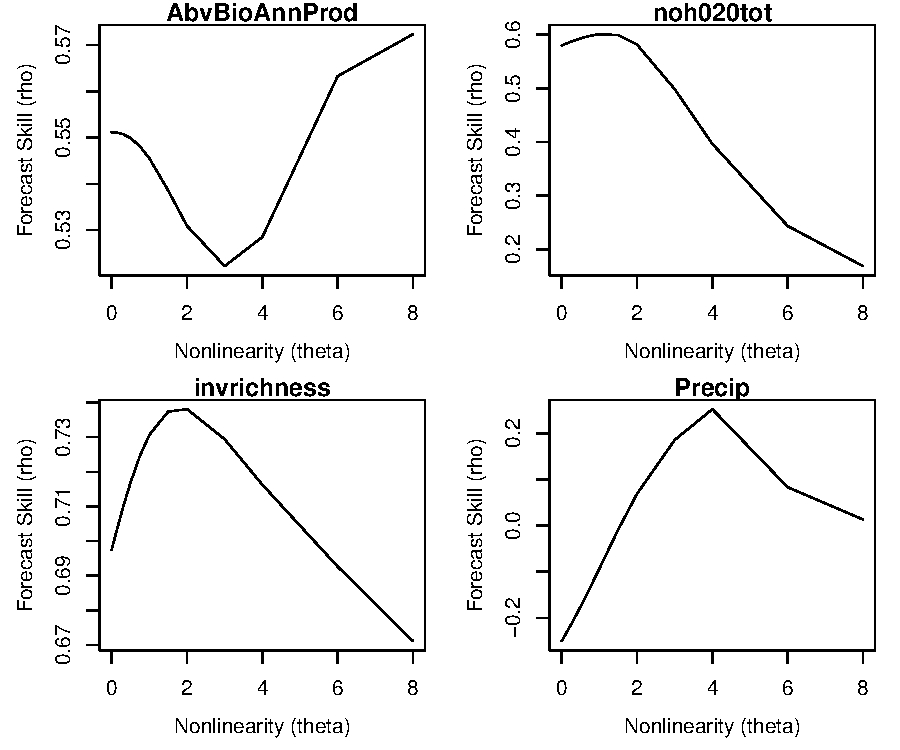
\includegraphics[width=\maxwidth{\textwidth}]{fig_redm_10.pdf}\end{center}
\caption[Nonlinearity of biological and physical variables in E120.]{\textbf{Nonlinearity of biological and physical variables in E120.}\newline
Both biological time series (``AbvBioAnnProd'' and ``invrichness'') show nonlinearity, with improved forecast skill for $\theta > 0$ compared to forecast skill at $\theta = 0$. Soil nitrate levels (``noh020tot'') and precipitation (``Precip''), also appear to be nonlinear. (Note that in this case, the S-map model for precipitation shows positive forecast skill when $\theta > 0$, indicating that there may be some (nonlinear) predictability, in contrast to the simplex projection results in Figure \ref{fig_e120_simplex}.}
\end{figure}

Note that all time series suggest nonlinear dynamics in the data (because of the initial rise in rho for non-zero theta, followed by a sharp drop-off in rho with theta).

\subsection{Multivariate Models}

Next, we can use information from several time series to make better predictions about system dynamics. We can accomplish this with the \lstinline{block_lnlp} command. First, we need to manually construct lagged vectors for each variable. This requires a bit of care in coding, as we need to ensure that lagged components come only from observations within a single field and transect.

\begin{lstlisting}
n <- NROW(composite_ts)

# make lags
block_data <- data.frame(year=composite_ts$year)
block_data$AB_tm <- composite_ts$AbvBioAnnProd
block_data$AB_tm1 <- c(NA, block_data$AB_tm[-n])
block_data$AB_tm2 <- c(NA, block_data$AB_tm1[-n])
block_data$AB_tm3 <- c(NA, block_data$AB_tm2[-n])

block_data$NO_tm <- composite_ts$noh020tot
block_data$NO_tm1 <- c(NA, block_data$NO_tm[-n])
block_data$NO_tm2 <- c(NA, block_data$NO_tm1[-n])
block_data$NO_tm3 <- c(NA, block_data$NO_tm2[-n])

block_data$IV_tm <- composite_ts$invrichness
block_data$IV_tm1 <- c(NA, block_data$IV_tm[-n])
block_data$IV_tm2 <- c(NA, block_data$IV_tm1[-n])
block_data$IV_tm3 <- c(NA, block_data$IV_tm2[-n])

block_data$PR_tm <- composite_ts$SummerPrecip.mm
block_data$PR_tm1 <- c(NA, block_data$PR_tm[-n])
block_data$PR_tm2 <- c(NA, block_data$PR_tm1[-n])
block_data$PR_tm3 <- c(NA, block_data$PR_tm2[-n])

# remove overlaps from other plots
startyear <- 1996
for(i in 2:nrow(block_data)) {
    if(block_data$year[i] < block_data$year[i-1]) {
        startyear <- block_data$year[i]
        }
    if(block_data$year[i] == startyear) {
        block_data[i,c("AB_tm1", "NO_tm1", "IV_tm1", "PR_tm1")] <- NA
        block_data[i,c("AB_tm2", "NO_tm2", "IV_tm2", "PR_tm2")] <- NA
        block_data[i,c("AB_tm3", "NO_tm3", "IV_tm3", "PR_tm3")] <- NA
        }
    if(block_data$year[i] == (startyear+1)) {
        block_data[i,c("AB_tm2", "NO_tm2", "IV_tm2", "PR_tm2")] <- NA
        block_data[i,c("AB_tm3", "NO_tm3", "IV_tm3", "PR_tm3")] <- NA
        }
    if(block_data$year[i] == (startyear+2)) {
        block_data[i,c("AB_tm3", "NO_tm3", "IV_tm3", "PR_tm3")] <- NA
        }
    }
head(block_data[,1:5],20)
\end{lstlisting}

\begin{lstlisting}[backgroundcolor=\color{white}, commentstyle=\ttfamily]
##    year      AB_tm     AB_tm1     AB_tm2     AB_tm3
## 1  1996 -1.0626351         NA         NA         NA
## 2  1997 -0.5456990 -1.0626351         NA         NA
## 3  1998  1.6338642 -0.5456990 -1.0626351         NA
## 4  1999 -0.4869863  1.6338642 -0.5456990 -1.0626351
## 5  2001 -0.2983658 -0.4869863  1.6338642 -0.5456990
## 6  2002  0.7598219 -0.2983658 -0.4869863  1.6338642
## 7  1996 -1.0139507         NA         NA         NA
## 8  1997 -0.9855735 -1.0139507         NA         NA
## 9  1998  1.4960850 -0.9855735 -1.0139507         NA
## 10 1999  0.3898716  1.4960850 -0.9855735 -1.0139507
## 11 2001 -0.4926840  0.3898716  1.4960850 -0.9855735
## 12 2002  0.6062517 -0.4926840  0.3898716  1.4960850
## 13 1996 -1.4989147         NA         NA         NA
## 14 1997 -0.6867934 -1.4989147         NA         NA
## 15 1998  1.5499186 -0.6867934 -1.4989147         NA
## 16 1999  0.3648442  1.5499186 -0.6867934 -1.4989147
## 17 2000  0.6089230  0.3648442  1.5499186 -0.6867934
## 18 2001 -0.5679305  0.6089230  0.3648442  1.5499186
## 19 2002  0.2299527 -0.5679305  0.6089230  0.3648442
## 20 1996 -1.3230421         NA         NA         NA
\end{lstlisting}

Now, we can run \lstinline{block_lnlp} on the composite, multi-variate time series. First, we run the algorithm to predict primary productivity dynamics, based on its own lagged dynamics. Next, we add additional information about precipitation:

\begin{lstlisting}
block_lnlp_output_AB <- block_lnlp(block_data, lib = composite_lib, pred = composite_pred, columns = c("AB_tm", "AB_tm1", "AB_tm2"), target_column = 1, stats_only = FALSE, first_column_time = TRUE)

block_lnlp_output_ABPR <- block_lnlp(block_data, lib = composite_lib, pred = composite_pred, columns = c("AB_tm", "AB_tm1", "AB_tm2", "PR_tm", "PR_tm1", "PR_tm2"), target_column = 1, stats_only = FALSE, first_column_time = TRUE)
\end{lstlisting}

Note that each additional variable adds slightly to the predictive power of the model.

\begin{lstlisting}
observed_AB <- block_lnlp_output_AB[[1]]$model_output$obs
predicted_AB <- block_lnlp_output_AB[[1]]$model_output$pred

observed_ABPR <- block_lnlp_output_ABPR[[1]]$model_output$obs
predicted_ABPR <- block_lnlp_output_ABPR[[1]]$model_output$pred

par(mar = c(4,4,1,1), pty = "s", mgp = c(2.5, 1, 0), mfrow = c(1,2))
plot_range <- range(c(observed_AB, predicted_AB), na.rm = TRUE)
plot(observed_AB, predicted_AB, xlim = plot_range, ylim = plot_range, xlab = "Observed", ylab = "Predicted", main = "Productivity (Univariate Model)")
abline(a = 0, b = 1, lty = 2, col = "darkgrey", lwd=2)
abline(lm(predicted_AB~observed_AB), col="black", lty=3, lwd=2)

plot(observed_ABPR, predicted_ABPR, xlim = plot_range, ylim = plot_range, xlab = "Observed", ylab = "Predicted", main = "Productivity (Multivariate Model)", pch=2, col="red")
abline(a = 0, b = 1, lty = 2, col = "darkgrey", lwd=2)
abline(lm(predicted_ABPR~observed_ABPR), col="red", lty=3, lwd=2)
\end{lstlisting}

\begin{figure}[!ht]
\begin{center}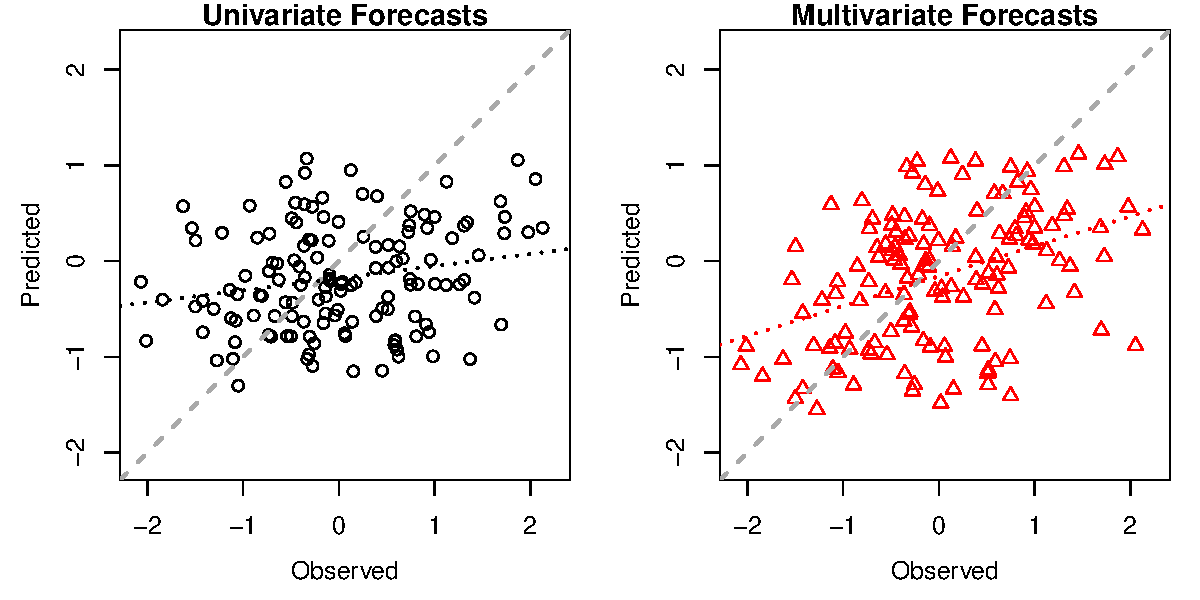
\includegraphics[width=\maxwidth{\textwidth}]{fig_redm_11.pdf}\end{center}
\caption[Comparison of univariate and multivariate forecasts of annual aboveground productivity.]{\textbf{Comparison of univariate and multivariate forecasts of annual aboveground productivity.}\newline
Points are actual predictions, black and red dotted lines are the lines of best fit, and the dark grey dashed lines Including lags of precipitation appears to improve predictions of productivity, with better coherence between observations and predictions for the multivariate model.}
\end{figure}

\subsection{Convergent Cross Mapping}

Finally, we can apply CCM to our data in order to test for causal links among variables.

In each case, we use the embedding dimension corresponding to the ``best'' embedding dimension for the variable that we are trying to predict (i.e., the putative causal process).

\begin{lstlisting}
# A. repens:
no_xmap_inv <- ccm(composite_ts, lib=segments, pred=segments, E = bestE[4], lib_column = "noh020tot", target_column = "invrichness", lib_sizes = c(seq(5, 55, by=2), seq(55, 400, by=50)), num_samples = 100, silent = TRUE)
inv_xmap_no <- ccm(composite_ts, lib=composite_lib, pred=composite_pred, E = bestE[1], lib_column = "invrichness", target_column = "noh020tot", lib_sizes = c(seq(5, 55, by=2), seq(55, 400, by=50)), num_samples = 100, silent = TRUE)

n_xmap_i_means <- data.frame(ccm_means(no_xmap_inv), sd.rho = with(no_xmap_inv, tapply(rho, lib_size, sd)))
i_xmap_n_means <- data.frame(ccm_means(inv_xmap_no), sd.rho = with(inv_xmap_no, tapply(rho, lib_size, sd)))

# S. scoparium:
ab_xmap_inv <- ccm(composite_ts, lib=segments, pred=segments, E = bestE[4], lib_column = "AbvBioAnnProd", target_column = "invrichness", lib_sizes = c(seq(5, 55, by=2), seq(55, 400, by=50)), num_samples = 100, silent = TRUE)
inv_xmap_ab <- ccm(composite_ts, lib=segments, pred=segments, E = bestE[2], lib_column = "invrichness", target_column = "AbvBioAnnProd", lib_sizes = c(seq(5, 55, by=2), seq(55, 400, by=50)), num_samples = 100, silent = TRUE)

a_xmap_i_means <- data.frame(ccm_means(ab_xmap_inv), sd.rho=with(ab_xmap_inv, tapply(rho, lib_size, sd)))
i_xmap_a_means <- data.frame(ccm_means(inv_xmap_ab), sd.rho=with(inv_xmap_ab, tapply(rho, lib_size, sd)))

# plot output
par(mar = c(4,4,1,1))
plot(n_xmap_i_means$lib_size, pmax(0, n_xmap_i_means$rho), type = "l", col = "red", xlab = "Library Size", ylab = "Cross Map Skill (rho)", ylim = c(0, 0.6), lwd=2)
lines(i_xmap_n_means$lib_size, pmax(0, i_xmap_n_means$rho), col = "blue", lwd=2)
legend(x = "topleft", legend = c("Nitrate xmap Inv. Richness", "Inv. Richness xmap Nitrate"), col = c("red", "blue"), lwd = 2, inset = 0.02, bty="n", cex = 0.8)
abline(h=0, lty=3, col="darkgrey", lwd=2)

# add CIs
lines(n_xmap_i_means$lib_size, n_xmap_i_means$rho+n_xmap_i_means$sd.rho, col = "red", lty=2, lwd=2)
lines(n_xmap_i_means$lib_size, n_xmap_i_means$rho-n_xmap_i_means$sd.rho, col = "red", lty=2, lwd=2)
lines(i_xmap_n_means$lib_size, i_xmap_n_means$rho+i_xmap_n_means$sd.rho, col = "blue", lty=2, lwd=2)
lines(i_xmap_n_means$lib_size, i_xmap_n_means$rho-i_xmap_n_means$sd.rho, col = "blue", lty=2, lwd=2)

plot(a_xmap_i_means$lib_size, pmax(0, a_xmap_i_means$rho), type = "l", col = "orange", xlab = "Library Size", ylab = "Cross Map Skill (rho)", ylim = c(0, 0.6), lwd=2)
lines(i_xmap_a_means$lib_size, pmax(0, i_xmap_a_means$rho), col = "blue", lwd=2)
legend(x = "topleft", legend = c("Abv. Biomass xmap Inv. Richness", "Inv. Richness xmap Abv. Biomass"), col = c("orange", "blue"), lwd = 2, inset = 0.02, bty="n", cex = 0.8)
abline(h=0, lty=3, col="darkgrey", lwd=2)

# add CIs
lines(a_xmap_i_means$lib_size, a_xmap_i_means$rho+a_xmap_i_means$sd.rho, col = "orange", lty=2, lwd=2)
lines(a_xmap_i_means$lib_size, a_xmap_i_means$rho-a_xmap_i_means$sd.rho, col = "orange", lty=2, lwd=2)
lines(i_xmap_a_means$lib_size, i_xmap_a_means$rho+i_xmap_a_means$sd.rho, col = "blue", lty=2, lwd=2)
lines(i_xmap_a_means$lib_size, i_xmap_a_means$rho-i_xmap_a_means$sd.rho, col = "blue", lty=2, lwd=2)
\end{lstlisting}

\begin{figure}[!ht]
\begin{center}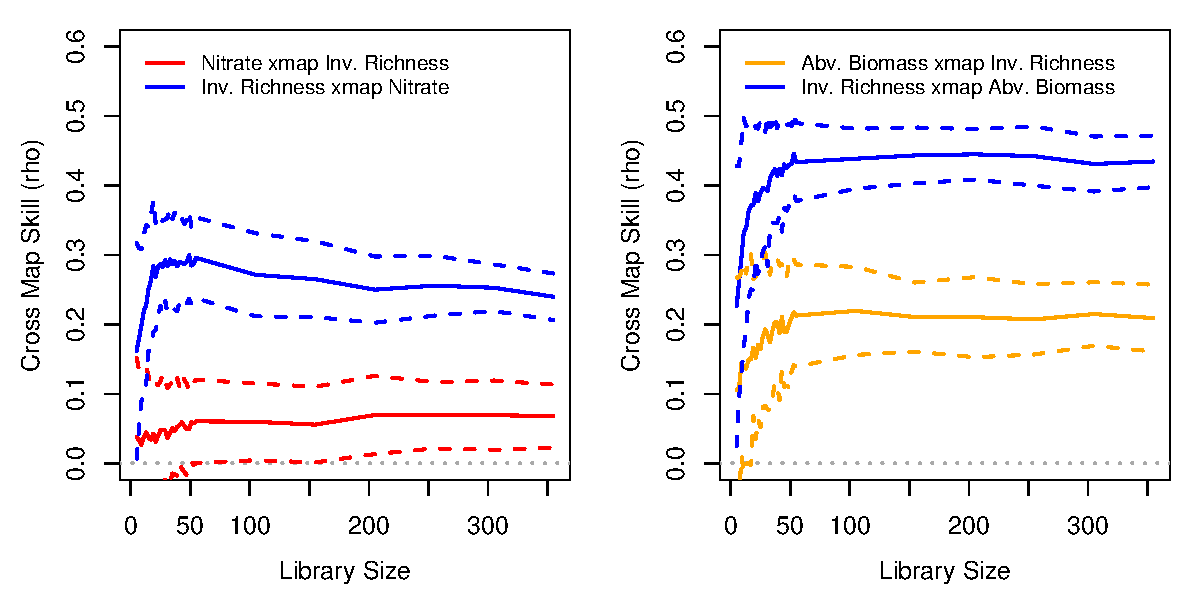
\includegraphics[width=\maxwidth{\textwidth}]{fig_redm_12.pdf}\end{center}
\caption[Causal drivers of species richness.]{\textbf{Causal drivers of species richness.}\newline
Convergent cross mapping (CCM) between species richness and nitrate (left panel) suggests a causal effect of nitrate on species richness, but no effect in the opposite direction. In contrast, CCM between species richness and productivity indicates causal effects in both directions.}
\end{figure}

In each case, results suggest that invasive richness is driven by other variables more strongly than it influences them in return. In particular, while invasion dynamics appear to be strongly forced by soil nitrate dynamics, invasion does not appear influence plot soil nitrate at all. This makes sense, as invading species in these plots are quickly weeded out and should not have time to influence local environmental conditions. Causal forcing between biomass and invasion, on the other hand, may be bi-directional based on our analyses. Again, though, it makes sense that there should only be moderate effects of invading species on plot-level biomass (e.g., by decreasing biomass of planted species through light competition), while effects of plot-level planted biomass on invader success should be much stronger (e.g., through competition for space or soil resources).

\section{Example 2: Apple-Blossom Thrips}

In this next example, we will use EDM methods to re-examine the classic apple-blossom thrips (\emph{Thrips imaginis}) time series from the Wait Institute in Australia \cite{Davidson_1948, Davidson_1948a}. Seasonal outbreaks of \emph{Thrips imaginis} were observed to vary greatly in magnitude from year to year, but large outbreaks tended to coincide across large spatial domains. This lead to the hypothesis that regional-scale climatic factors were responsible for controlling the size of the seasonal outbreaks (what might now be called the Moran effect).

\begin{lstlisting}
data(thrips_block)
colnames(thrips_block)
\end{lstlisting}

\begin{lstlisting}[backgroundcolor=\color{white}, commentstyle=\ttfamily]
## [1] "Year"      "Month"     "Thrips_imaginis" "maxT_degC"     "Rain_mm"        
## [6] "Season" 
\end{lstlisting}

The first data column \lstinline{colnames(thrips_block)[3]} contains counts of \emph{Thrips imaginis} obtained from the Global Population Dynamics Database. \lstinline{colnames(thrips_block)[4]} is the mean maximum daily temperature (degrees F) taken over each month and \lstinline{colnames(thrips_block)[5]} is the monthly rainfall (mm), both from the Waite Institute. The final column \lstinline{colnames(thrips_block)[6]} is a simple annual sinusoid that peaks in December (the Austral summer) that acts as an indicator of season.

First, we plot the data.

\begin{lstlisting}
par(mar = c(4,4,1,1), mfrow = c(4,1), mgp = c(2.5,1,0))
time_dec <- thrips_block$Year + (thrips_block$Month)/12
plot(time_dec, thrips_block$Thrips_imaginis, type = "l", col = "green", ylab = "Thrips")
plot(time_dec, thrips_block$maxT_degC, type = "l", col = "red", ylab = "maxT (oC)")
plot(time_dec, thrips_block$Rain_mm, type = "l", col = "blue", ylab = "Rain (mm)")
plot(time_dec, thrips_block$Season, type = "l", col = "magenta", ylab = "Season")
\end{lstlisting}

\begin{figure}[!ht]
\begin{center}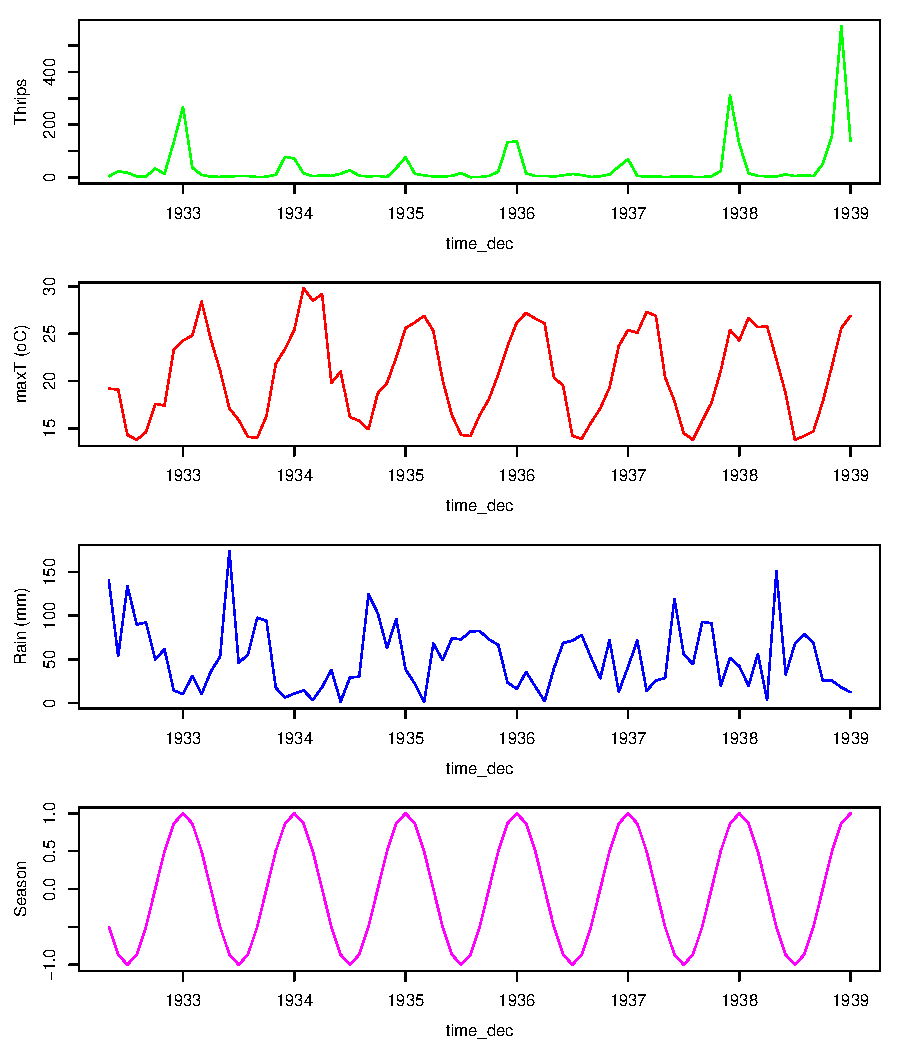
\includegraphics[width=\maxwidth{\textwidth}]{fig_redm_13.pdf}\end{center}
\caption[Time series of Apple-Blossom Thrips.]{\textbf{Time series of Apple-Blossom Thrips.}\newline
Time series for thrips abundance (green), maximum daily temperature (red), monthly rainfall (blue), and season (magenta). Note that all the time-series variables, particularly the mean maximum daily Temperature, show marked seasonality.}
\end{figure}

\subsection{Univariate Analysis}

\begin{lstlisting}
ts <- thrips_block$Thrips_imaginis
lib <- c(1, length(ts))
pred <- c(1, length(ts))
simplex_output <- simplex(ts, lib, pred, tau = 1)

par(mar = c(4,4,1,1), mgp = c(2.5, 1, 0))
plot(simplex_output$E, simplex_output$rho, type = "l", xlab = "Embedding Dimension (E)", ylab = "Forecast Skill (rho)")
\end{lstlisting}

\begin{figure}[!ht]
\begin{center}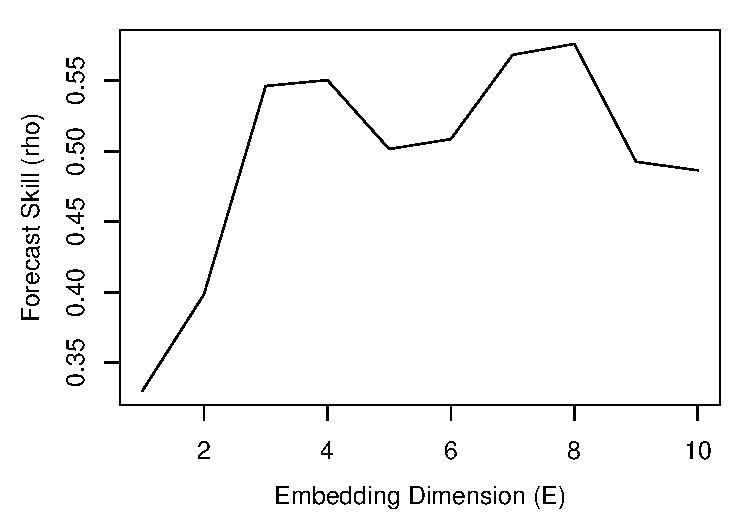
\includegraphics[width=\maxwidth{\textwidth}]{fig_redm_14.pdf}\end{center}
\caption[Predictability of Apple-Blossom Thrips.]{\textbf{Predictability of Apple-Blossom Thrips.}\newline
Plotting forecast skill ($\rho$) vs. embedding dimension ($E$) indicates predictable dynamics. While there is an initial peak in the forecast skill at $E = 4$, the global maximum is at $E = 8$. This suggests that both $E = 4$ and $E = 8$ are practical embedding dimensions.}
\end{figure}

To test for nonlinearity, we examine both $E = 4$ and $E = 8$ to verify that the S-maps result is robust to the choice of embedding dimension.

\begin{lstlisting}
smap_output <- list()
smap_output[[1]] <- s_map(ts, lib, pred, E = 4)
smap_output[[2]] <- s_map(ts, lib, pred, E = 8)

par(mar = c(4,4,1,1), mgp = c(2.5, 1, 0))
plot(smap_output[[1]]$theta, smap_output[[1]]$rho, type = "l", xlim=c(0,4), ylim = c(0.2, 0.6), xlab = "Nonlinearity (theta)", ylab = "Forecast Skill (rho)", col = "blue")
lines(smap_output[[2]]$theta, smap_output[[2]]$rho, col = "red")
legend("topright", legend = c("E = 4", "E = 8"), col = c("blue", "red"), lwd = 1)
\end{lstlisting}

\begin{figure}[!ht]
\begin{center}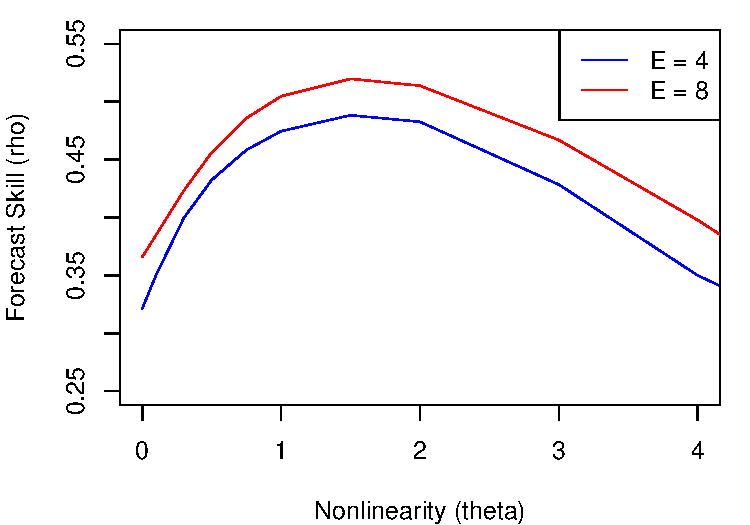
\includegraphics[width=\maxwidth{\textwidth}]{fig_redm_15.pdf}\end{center}
\caption[Nonlinearity of Apple-Blossom Thrips.]{\textbf{Nonlinearity of Apple-Blossom Thrips.}\newline
Plotting forecast skill ($\rho$) vs. nonlinearity (theta) demonstrates clear nonlinear dynamics. At both $E = 4$ (blue) and "E = 8" (red), nonlinear models ($\theta > 0$) produce better predictions than the equivalent linear model ($\theta = 0$).}
\label{fig_redm_thrips_smap}
\end{figure}

The S-map (Figure \ref{fig_redm_thrips_smap}) results demonstrate clear nonlinearity in the Thrips time series. This suggests that Thrips, despite the strong seasonal dynamics, do not simply track the environment passively, but have some intrinsic dynamics. To look more closely at the issue of seasonal drivers, however, we turn to convergent cross-mapping (CCM).

\subsection{Seasonal Drivers}

Recall that there is a two-part criterion for CCM to be a rigorous test of causality. (1) The cross-map prediction skill with the full time-series is statistically significant. (2) Cross-map prediction demonstrates convergence, i.e. prediction skill increases as more of the time-series is used. 

\subsubsection{Cross-map matrix}

For an initial summary, we first simply compute the cross-map skill (measured with Pearson's $\rho$) with the full time-series.

\begin{lstlisting}
ncol <- dim(thrips_block)[2]-2
M_rho <- array(NA,dim=c(ncol,ncol),dimnames=list(colnames(thrips_block[3:6]),colnames(thrips_block[3:6])))

for (i in 1:ncol){
    for (j in 1:ncol){
        if (i!=j){
            out_temp <- ccm(thrips_block,E=8,lib_column=2+i,target_column=2+j,
                            lib_sizes = dim(thrips_block)[1],replace=FALSE, silent = TRUE)
            M_rho[i,j] <- out_temp$rho
            } 
        }
    }
\end{lstlisting}

\subsubsection{Correlation matrix}

For comparison we also compute the lag cross-correlation, allowing lags up to $\pm 6$ months.
\begin{lstlisting}
M_corr <- array(NA,dim=c(ncol,ncol),dimnames=list(colnames(thrips_block[3:6]),colnames(thrips_block[3:6])))

for (i in 1:ncol){
    for (j in 1:ncol){
        if (i!=j){
            cf_temp <- ccf(x=thrips_block[,2+i], y=thrips_block[,2+j], type = "correlation", lag.max = 6, plot = FALSE)$acf
            M_corr[i,j] <- max(abs(cf_temp))
            }
        }
}
\end{lstlisting}

We compare the two matrices.

\textbf{Cross-map}
\begin{lstlisting}
M_rho
\end{lstlisting}

\begin{lstlisting}[backgroundcolor = \color{white}, commentstyle = \ttfamily]
##                 Thrips_imaginis maxT_degC   Rain_mm    Season
## Thrips_imaginis              NA 0.9239205 0.5136489 0.9551902
## maxT_degC             0.6046406        NA 0.4629704 0.9918832
## Rain_mm               0.4277785 0.8210977        NA 0.7780148
## Season                0.5619095 0.9625766 0.3944837        NA
\end{lstlisting}

\textbf{Correlation}
\begin{lstlisting}
M_corr
\end{lstlisting}

\begin{lstlisting}[backgroundcolor = \color{white}, commentstyle = \ttfamily]
##                 Thrips_imaginis maxT_degC   Rain_mm    Season
## Thrips_imaginis              NA 0.4489876 0.2668395 0.4488334
## maxT_degC             0.4489876        NA 0.5949077 0.9452625
## Rain_mm               0.2668395 0.5949077        NA 0.5332935
## Season                0.4488334 0.9452625 0.5332935        NA
\end{lstlisting}

Notice that the lagged correlation between $maxT$ and the seasonal indicator is extremely high, and $Season$ can almost perfectly cross-map $maxT$, $\rho =$ \lstinline{r M_rho["Season", "maxT_degC"]}. This makes the interpretation of cross-mapping more complicated, because we have to consider synchrony. Let's elaborate. It is clear from cross-mapping (or even just visual inspection) that seasonality drives Thrips abundance. Since the monthly mean maximum temperature is almost perfectly synchronized to the seasons, it contains the same information as the simple season indicator. Any variable that can predict (cross-map) the seasonal cycle, i.e. was influenced by seasonality, will therefore also predict $maxT$, regardless of if temperature is actually the mechanism of seasonal forcing.

\subsubsection{Convergent Cross-Mapping}

With this in mind, we examine convergence in cross-map predictability.

\begin{lstlisting}
thrips_xmap_maxT <- ccm(thrips_block, E = 8, random_libs = TRUE, lib_column = "Thrips_imaginis", target_column = "maxT_degC", lib_sizes = seq(10, 75, by = 5), num_samples = 300)
maxT_xmap_thrips <- ccm(thrips_block, E = 8, random_libs = TRUE, lib_column = "maxT_degC", target_column = "Thrips_imaginis", lib_sizes = seq(10, 75, by = 5), num_samples = 300)

thrips_xmap_Rain <- ccm(thrips_block, E = 8, random_libs = TRUE, lib_column = "Thrips_imaginis", target_column = "Rain_mm", lib_sizes = seq(10, 75, by = 5), num_samples = 300)
Rain_xmap_thrips <- ccm(thrips_block, E = 8, random_libs = TRUE, lib_column = "Rain_mm", target_column = "Thrips_imaginis", lib_sizes = seq(10, 75, by = 5), num_samples = 300, silent = TRUE)

thrips_xmap_Season <- ccm(thrips_block, E = 8, random_libs = TRUE, lib_column = "Thrips_imaginis", target_column = "Season", lib_sizes = seq(10, 75, by = 5), num_samples = 300)
Season_xmap_thrips <- ccm(thrips_block, E = 8, random_libs = TRUE, lib_column = "Season", target_column = "Thrips_imaginis", lib_sizes = seq(10, 75, by = 5), num_samples = 300)

xmap_means_maxT <- list(ccm_means(thrips_xmap_maxT),ccm_means(maxT_xmap_thrips))
xmap_means_Rain <- list(ccm_means(thrips_xmap_Rain),ccm_means(Rain_xmap_thrips))
xmap_means_Season <- list(ccm_means(thrips_xmap_Season), ccm_means(Season_xmap_thrips))
\end{lstlisting}

Next, we plot the cross map skill ($\rho$) against the library size ($L$):

\begin{lstlisting}
par(mar = c(4,4,1,1), mgp = c(2.5, 1, 0), mfrow = c(2,2))
plot(xmap_means_maxT[[1]]$lib_size, pmax(0, xmap_means_maxT[[1]]$rho), type = "l", col = "red",  xlab = "Library Size", ylab = "Cross Map Skill (rho)", ylim = c(0.2, 1))
lines(xmap_means_maxT[[2]]$lib_size, pmax(0, xmap_means_maxT[[2]]$rho), col = "green")
abline(h=M_corr["Thrips_imaginis", "maxT_degC"], col = "black", lty = 2)
legend(x = "bottomright", legend = c("Thrips xmap maxT", "maxT xmap Thrips"), col = c("red", "green"), lwd = 1, inset = 0.02)

plot(xmap_means_Rain[[1]]$lib_size, pmax(0, xmap_means_Rain[[1]]$rho), type = "l", col = "blue", xlab = "Library Size", ylab = "Cross Map Skill (rho)", ylim = c(0.1, 0.5))
lines(xmap_means_Rain[[2]]$lib_size, pmax(0, xmap_means_Rain[[2]]$rho), col = "green")
abline(h=M_corr["Thrips_imaginis", "Rain_mm"], col = "black", lty = 2)
legend(x = "bottomright", legend = c("Thrips xmap Rain", "Rain xmap Thrips"), 
 col = c("blue", "green"), lwd = 1, inset = 0.02)

plot(xmap_means_Season[[1]]$lib_size, pmax(0, xmap_means_Season[[1]]$rho), type = "l", col = "magenta", xlab = "Library Size", ylab = "Cross Map Skill (rho)", ylim = c(0.2, 1))
lines(xmap_means_Season[[2]]$lib_size, pmax(0, xmap_means_Season[[2]]$rho), col = "green")
abline(h=M_corr["Thrips_imaginis", "Season"], col = "black", lty = 2)
legend(x = "bottomright", legend = c("Thrips xmap Season", "Season xmap Thrips"), col = c("magenta", "green"), lwd = 1, inset = 0.02)
\end{lstlisting}

\begin{figure}[!ht]
\begin{center}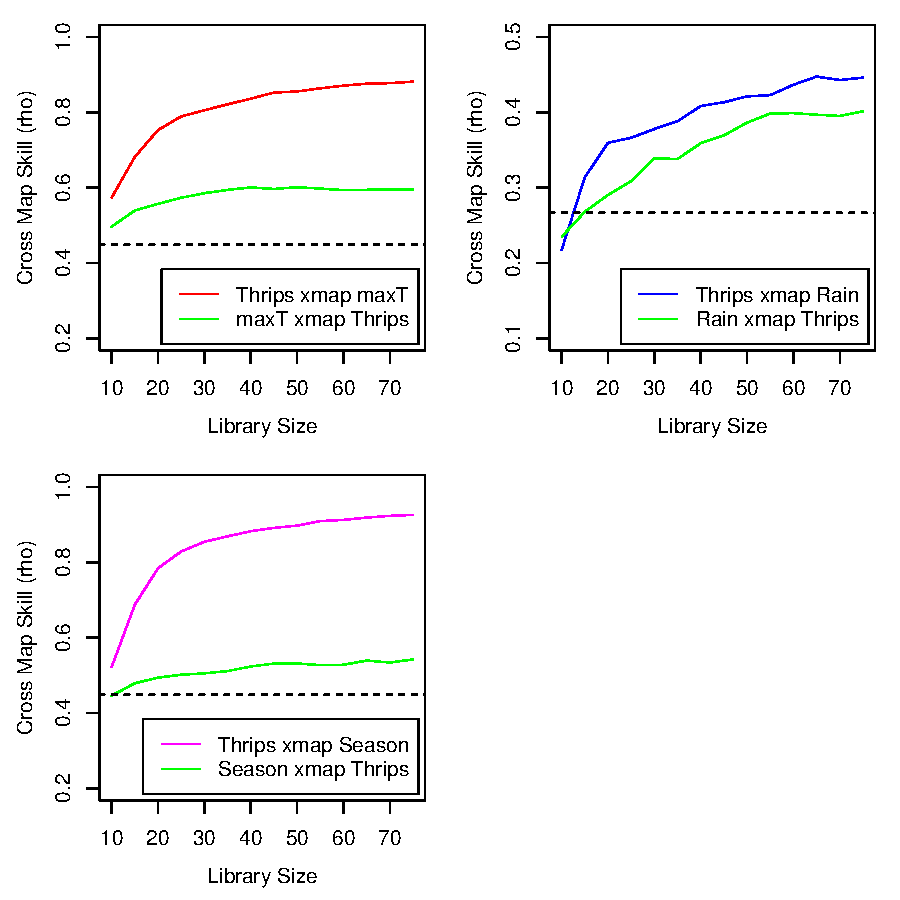
\includegraphics[width=\maxwidth{\textwidth}]{fig_redm_16.pdf}\end{center}
\caption[Cross mapping between Thrips abundance and potential drivers.]{\textbf{Cross mapping between Thrips abundance and potential drivers.}\newline
Cross mapping from Thrips to temperature (``Thrips xmap maxT'', red line) suggests a strong effect of temperature on Thrips abundance. In the opposite direction (``maxT xmap Thrips'', blue line), CCM suggests a weaker effect of Thrips on temperature. The same is true for rainfall, and the seasonal proxy. Cross-correlation between the variables is indicated by a black dashed line.}
\end{figure}

Importantly, the results show clear evidence of convergence for $Thrips$ cross-mapping the climactic variables, and the $\rho$ at maximum $L$ greatly exceeds the linear correlation. However, we are still left with the conundrum that $maxT$ and to a lesser extent $Rain$ are easily predicted from the seasonal cycle, suggesting that Thrips abundance affects temperature and rainfall. Since this is clearly false, it suggests that cross map skill is artificially high due to shared seasonal patterns, and $maxT$ and $Rain$ may only appear to affect $Thrips$ because of shared seasonal forcing.

To reframe, we would like to reject the null hypothesis that the causal effects we measure for $maxT$ and $Rain$ with CCM can be solely explained by their shared seasonality. This hypothesis is readily tested using surrogate methods.

\subsubsection{Seasonal Surrogate Test}

\begin{lstlisting}
num_surr <- 1000
surr_maxT <- make_surrogate_data(thrips_block$maxT_degC, method = "seasonal", T_period = 12, num_surr = num_surr)
surr_Rain <- make_surrogate_data(thrips_block$Rain_mm, method = "seasonal", T_period = 12, num_surr = num_surr)

rho_surr <- data.frame(maxT = numeric(num_surr), Rain = numeric(num_surr))

for (i in 1:num_surr) {
    rho_surr$maxT[i] <- ccm(cbind(thrips_block$Thrips_imaginis, surr_maxT[,i]), E = 8, lib_column = 1, target_column = 2, lib_sizes = NROW(thrips_block), replace = FALSE)$rho
    
    rho_surr$Rain[i] <- ccm(cbind(thrips_block$Thrips_imaginis, surr_Rain[,i]), E = 8, lib_column = 1, target_column = 2, lib_sizes = NROW(thrips_block), replace = FALSE)$rho
    }
\end{lstlisting}

We now have a null distribution, and can easily estimate the $p$ value for rejecting the null hypothesis of mutual seasonality. Here, the p-value is estimated as $\frac{k+1}{n+1}$, where $k$ is the number of ``successes'' (null values that exceed the true cross map skill), and $n$ is the number of null values computed.

\begin{lstlisting}
(sum(rho_surr$Rain > M_rho["Thrips_imaginis", "Rain_mm"]) + 1) / (length(rho_surr$Rain) + 1)
\end{lstlisting}

\begin{lstlisting}[backgroundcolor = \color{white}, commentstyle = \ttfamily]
## [1] 0.05494505
\end{lstlisting}

\begin{lstlisting}
(sum(rho_surr$maxT > M_rho["Thrips_imaginis", "maxT_degC"]) + 1) / (length(rho_surr$maxT) + 1)
\end{lstlisting}

\begin{lstlisting}[backgroundcolor = \color{white}, commentstyle = \ttfamily]
## [1] 0.1748252
\end{lstlisting}

In both cases, the CCM we measure for the real time series are better than the median expectation under the null hypothesis. For rainfall, the effect is not significant based on the common threshold of $p < 0.05$, but is marginally significant using the threshold of $p < 0.10$. However, the high correlation between the maximum daily temperature averaged over a month and the seasonal cycle makes it harder to establish significance for the effect of $maxT$. We note that the original Thrips data collections were at a much higher frequency than those available through the GPDD, and that $maxT$ shows much larger departures from the seasonal cycle on shorter time-scales. With more highly resolved data, it may well be possible to establish significance, by increasing the power of our tests.

\section{Technical Details}

\subsection{Data Input}

The rEDM functions are designed to accept data in common R data formats, namely vectors, matrices, and data.frames. Depending on the specific function, one or the other data type is preferred. Please see the documentation associated with individual functions for more details.

Missing data can be input using either \lstinline{NA} or \lstinline{NAN}. The program will automatically ignore such missing values as appropriate. For instance, simplex projection will not select nearest neighbors if any of the state vector coordinates is missing or if the corresponding target value is missing.

Note that when there is no observed target value, it is still possible to predict from a given state vector, if it has no missing values. Thus, it is possible to use the software to forecast ahead from an observed state into an unobserved future. This can be done simply by substituting \lstinline{NA} or \lstinline{NAN} for unknown future values. However, be aware that the performance metrics will be computed so as to ignore such predictions (since there are no observed values to compare against). Thus, the statistics (e.g., $\rho$, MAE, RMSE) may be computed based on fewer predictions than those actually made by the software.

\subsection{General Function Arguments}

Many of the functions in rEDM are designed around the same prediction engine, and so share many of the same arguments. Please see the documentation associated with individual functions to verify which parameters are applicable as well as the default values (which can change, depending on which function is called).

\begin{itemize}
\item lib
	\begin{itemize}
    	\item a 2-column matrix (or 2-element vector) where each row specifies the portions of the time series to use for attractor reconstruction (i.e., the set of vectors that can be selected as nearest neighbors)
	\item e.g., \lstinline{lib = c(1, n)} specifies that the first \lstinline{n} \emph{rows} of data are a contiguous time series block, each point of which can be used to construct state vectors
	\item by default, uses the entire input as a single contiguous segment
	\end{itemize}
\item pred
	\begin{itemize}
	\item (same format as lib, but specifies the portions of the time series to make predictions for)
	\end{itemize}
\item norm\_type
	\begin{itemize}
	\item \lstinline{"L2 norm"} (default) or \lstinline{"L1 norm"}: specifies which distance metric to use when doing calculations
	\item \lstinline{"L2 norm"} is the standard Euclidean distance, where the distance between a vector $\vec{x} = \langle x_1, x_2, \dots, x_n \rangle$ and $\vec{y} = \langle y_1, y_2, \dots, y_n \rangle$ is computed as $\sqrt{(x_1 - y_1)^2 + (x_2 - y_2)^x + \dots + (x_n - y_n)^2}$.
	\item \lstinline{"L1 norm"} is the Manhattan norm (also known as taxicab distance), where the distance between a vector $\vec{x} = \langle x_1, x_2, \dots, x_n \rangle$ and $\vec{y} = \langle y_1, y_2, \dots, y_n \rangle$ is computed as $|x_1 - y_1| + |x_2 - y_2| + \dots + |x_n - y_n|$.
	\end{itemize}
\item E
	\begin{itemize}
	\item the embedding dimension to use for attractor reconstruction
	\end{itemize}
\item tau
	\begin{itemize}
	\item the lag to use for attractor reconstruction; by default, set to 1
	\end{itemize}
\item tp
	\begin{itemize}
	\item the prediction horizon (how many steps ahead to make forecasts)
	\item negative values will also work
	\end{itemize}
\item num\_neighbors
	\begin{itemize}
	\item the number of neighbors to use
	\item \lstinline{"e+1"}, \lstinline{"E+1"}, \lstinline{"e + 1"}, and \lstinline{"E + 1"} will all peg this parameter to be `E+1` for each run
	\item values less than 1 will use all possible neighbors
	\end{itemize}
\item theta
	\begin{itemize}
	\item the nonlinear tuning parameter (for use with S-maps) that adjusts how distance is factored into computation of the local linear map (0 corresponds to a globally linear map, while values greater than 0 correspond to nonlinear models where the local linear map changes as a function of state-space)
	\end{itemize}
\item stats\_only
	\begin{itemize}
	\item \lstinline{TRUE} (default) or \lstinline{FALSE}: specifies whether the output should just contain statistics of the predictions, or also contain all the predictions that were made
	\end{itemize}
\item exclusion\_radius
	\begin{itemize}
	\item sets the threshold whereby all vectors with time indices too close to the predictee will be excluded from being considered nearest neighbors
	\item e.g., \lstinline{1} means that vectors must have an associated time index more than 1 away from potential nearest neighbors
	\item by default, set to NULL (turning this filtering off)
	\end{itemize}
\item epsilon
	\begin{itemize}
	\item sets the threshold whereby all vectors with distance too far away from the predictee will be excluded from being considered nearest neighbors
	\item e.g., \lstinline{epsilon = 2} means that vectors must have be within a distance of 2 from potential nearest neighbors
	\item by default, set to NULL (turning this filtering off)
	\end{itemize}
\item silent
	\begin{itemize}
	\item \lstinline{TRUE} or \lstinline{FALSE} (default): specifies whether to suppress warning messages from being printed to the R console
	\end{itemize}
\item save\_smap\_coefficients
	\begin{itemize}
	\item \lstinline{TRUE} or \lstinline{FALSE} (default): specifies whether to include a table of s-map coefficients with the output
	\item (note that setting this to \lstinline{TRUE} forces the full output as if \lstinline{stats_only = FALSE}, overriding the value for \lstinline{stats_only})
	\end{itemize}
\end{itemize}

\section{Applications}

\subsection{Composite Time Series}

In some cases, we may have multiple time series that can serve as spatial or ecological replicates. To treat these time series as replicates when applying EDM, we want to combine the data together into a single composite time series. Because the scale may differ across time series, we typically apply a normalization routine to linearly transform each time series to have mean = 0 and variance = 1 before concatenating. 

\begin{lstlisting}
data(sockeye_returns)

# separate time column from data
time <- sockeye_returns$year
sockeye_returns <- sockeye_returns[,-1]

# normalize each time series
n <- NCOL(sockeye_returns)
for(j in 1:n)
    {
    sockeye_returns[,j] <- (sockeye_returns[,j] - mean(sockeye_returns[,j])) / sd(sockeye_returns[,j])
    }

# make composite time series
composite_ts <- data.frame(year = time, 
                           returns = stack(sockeye_returns)$value)
\end{lstlisting}

Before applying EDM, however, we want to make sure that EDM will properly recognize the different time series segments as being different, so that lagged vectors are not constructed that contain coordinates spanning multiple time series. This is simply handled by constructing the \lstinline{lib} and \lstinline{pred} arguments so that the first column designates the start of each time series segment, and the second column designates the end.

\begin{lstlisting}
# make composite library
segments <- cbind(seq(from = 1, by = NROW(sockeye_returns), length.out = n),  seq(from = NROW(sockeye_returns), by = NROW(sockeye_returns), length.out = n))
composite_lib <- segments[1:5,]
composite_pred <- segments[6:9,]
\end{lstlisting}

We can then use the rEDM functions as normal:

\begin{lstlisting}
par(mar = c(4,4,1,1), mgp = c(2.5, 1, 0), mfrow = c(2,1))
simplex_output <- simplex(composite_ts, composite_lib, composite_pred)
plot(simplex_output$E, simplex_output$rho, type = "l",  xlab = "Embedding Dimension (E)", ylab = "Forecast Skill (rho)")

smap_output <- s_map(composite_ts, composite_lib, composite_pred, E = 8)
plot(smap_output$theta, smap_output$rho, type = "l", xlab = "Nonlinearity (theta)", ylab = "Forecast Skill (rho)")
\end{lstlisting}

\begin{figure}[!ht]
\begin{center}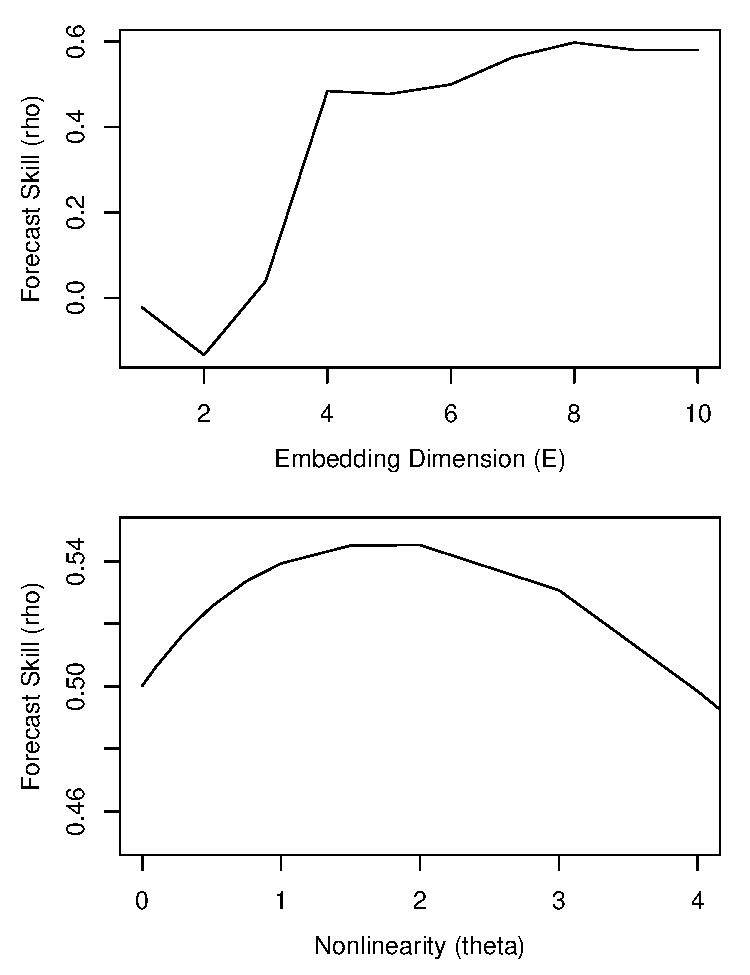
\includegraphics[width=\maxwidth{\textwidth}]{fig_redm_17.pdf}\end{center}
\caption[Univariate analysis of composite time series.]{\textbf{Univariate analysis of composite time series.}\newline
Simplex Projection indicates an optimal embedding dimension of 8. Using $E = 8$, an S-map analysis shows clear evidence of nonlinear dynamics.}
\end{figure}

\section{Acknowledgements}
The rEDM package is the latest incarnation of EDM code. Past versions have been developed by George Sugihara, Alan Trombla, Richard Penner, Victor Wong, Martin Casdagli, Mohsen Azarbayejani, Ava Pierce, Jennifer Trezzo, and Hao Ye.

This chapter contains material prepared for submission: Hao Ye, Adam T. Clark, and Ethan R. Deyle. rEDM: A package for empirical dynamic modeling based on attractor reconstruction. \emph{Journal of Statistical Software}. The dissertation author was the primary investigator and author of this paper.
